\section{Data illustrations\label{sec:results}} 
We apply the aforementioned models to simulated angular data. We then consider the analysis
    of atmospheric data. To tackle the difficult problem of assessing the convergence 
    an MCMC chain for a large-dimensional model, we monitor the log-posterior 
    density. In all the examples considered, MCMC samples produced stable traces of the
    log-posterior in less than 40 thousand  iterations. We use that as a burn-in, 
    and thereafter sample 10 thousand additional iterations. We then thin the chain by retaining one
    every ten samples, to obtain 1000 total samples. These are used to generate samples from the 
    posterior predictive densities. We used two different strategies to implement the MCMC samplers.
    For the models whose DP prior is centered around a log-normal distribution we used parallel 
    tempering. This serves to overcome the very slow mixing that we observed for these cases.
    The temperature ladder was set as $t_s = 1.3^{s}$,  for $s \in \lbrace0,1,\ldots,5\rbrace$. This was 
    set empirically in order to produce acceptable swap probabilities both for the simulated data, 
    and real data. Parallel tempering produces chains with good mixing properties, but has a 
    computational cost that  grows linearly with the number of temperatures. Thus, for the 
    gamma-centered models, we used a single chain. We leverage the fast speed of each iteration, 
    to obtain a large number of samples, that are appropriately thinned to deal with a mild
    autocorrelation. In summary, the strategy for log-normal centered models is based on a costly
    sampler with good mixing properties. The strategy for the gamma-centered models is based on
    a cheap sampler that can be run for a large number of iterations.

Our hyperprior parameters are set as follows: for the gamma-centered models (PG-G, PRG-G), 
    the shape parameter for the centering 
    distribution~$\xi_{\ell}\sim \mathcal{G}\left(1,1\right)$, and
    rate parameter~$\tau_{\ell}\sim\mathcal{G}\left(2,2\right)$.
    For the log-normal centered models (PG-LN, PRG-LN), the centering distribution's
    log-mean $\bm{\mu}\sim\mathcal{N}_d\left(0,\bm{I}_d\right)$, and covariance 
    matrix~$\Sigma\sim\mathcal{IW}\left(d + 10, (d+10)\bm{I}_{d}\right)$.  These values are 
    intended such that draws from the prior for $\Sigma$ will weakly tend towards the 
    identity matrix.
    For models learning rate parameters $\beta_{j\ell}$ (PG-G, PG-LN), the centering
    distribution's shape parameter $\zeta\sim\mathcal{G}\left(1,1\right)$ and rate parameter
    $\sigma\sim\mathcal{G}\left(2,2\right)$.  The choice of the $\mathcal{G}(2,2)$ for rate
    parameters places little mass near 0, in order to draw estimates for the value away from 
    0 for numerical stability.

\begin{algorithm} % algorithm using algorithm package
        \caption{Simulated Angular Dataset Generation Routine\label{algo:simulated}.
        $\mu_j$, $\Sigma_j$ are the parameters of the mixture component distribution; 
        $\pi$ is the probability vector assigning weight mixture components; $\delta_i$ 
        is the mixture component identifier for each simulated observation.}
        \begin{algorithmic}
        \For{$n_{\text{iter}}$ in $[1,\ldots,10]$}
        \For{$n_{\text{mix}}$ in $[1, 2, 4, 8]$}
            \For{$j$ in $1,\ldots,n_{\text{mix}}$}
                \State Generate $\mu_{j} \sim \mathcal{N}_{32}\left(\bm{0},\bm{I}\right)$
                \State Generate $\Sigma_{j}\sim\mathcal{IW}_{32}\left(70,70 \bm{I}\right)$
            \EndFor
            \State Generate $\pi\sim\text{Dirichlet}(\bm{10}_{n_{\text{mix}}})$
            \For{$i$ in $1,\ldots,1000$}
                \State Generate $\delta_i \sim \text{Categorical}(\pi)$
                \State Generate $\bm{X}_i \sim \mathcal{LN}\left(\mu_{[\delta_i]},\Sigma_{[\delta_i]}\right)$
            \EndFor
            \For{$n_{\text{col}}$ in $[2,4,8,16,24,32]$}
                \State Project columns 1 to $n_{\text{col}}$ of ${\bf X}$ onto $\mathcal{S}_{\infty}^{n_{\text{col}} - 1}$ and save.
            \EndFor
        \EndFor
        \EndFor
        \end{algorithmic}
    \end{algorithm}

\begin{figure}[t]
    \centering
    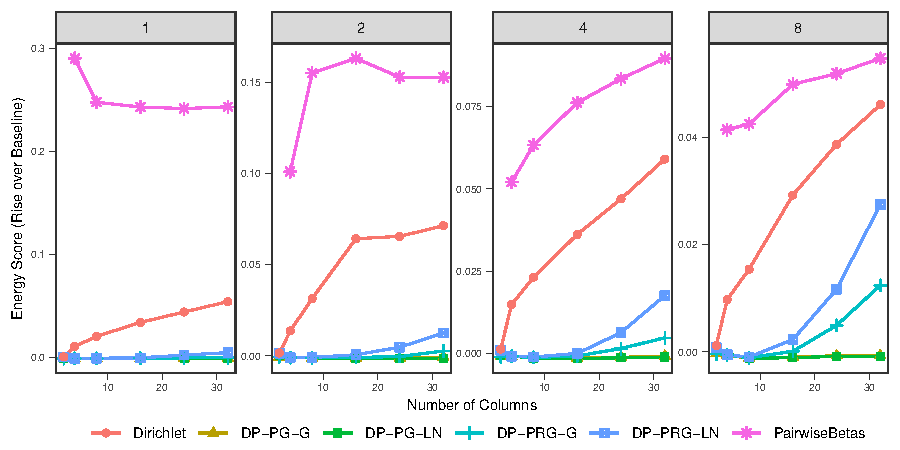
\includegraphics[height=2.5in, width = 0.9\textwidth]{./images/sim_es_rise}
    \caption{Average energy score rise over baseline (on $\mathbb{S}_{\infty}^{d-1}$) for various 
    models fitted to simulated data, with ascending count of mixture components (indicated by plot
    heading) and number of dimensions (indicated by horizontal axis).  Note that pairwise betas is
    a moment-restricted model.\label{fig:simpples}}
\end{figure}


\subsection{Simulation Study\label{subsec:simulated}}
The challenging problem in multivariate EVT is to capture the dependence 
    structure of the limiting distribution.  To this end, we focus our 
    simulation study specifically on the angular component.  To evaluate 
    our proposed approach for angular measure estimation 
    we consider simulated datasets on $\mathbb{S}_{\infty}^{d-1}$,
    for values of $d$ ranging between 2 and 32.  We generated each
    dataset as a mixture of multivariate log-normal distributions,
    projected onto $\mathbb{S}_{\infty}^{d-1}$. The generation 
    procedure is detailed in Algorithm~\ref{algo:simulated}. We produced 
    ten replicates of each configuration. We consider two gamma-centered
    and two log-normal centered DP mixture models, with and without restrictions in each
    case. To perform a comparative analysis we fitted 
   % \makenote{Comparative analysis using posterior predictive samples necessitates
    %alternative models having defined methods of sampling from their respective posterior
    %predictive distributions, for models defined on some normalization of the positive cone.  
    %To that end, we also consider the Dirichlet distribution, as well as} 
    %We also consider a Dirichlet distribution and 
    the pairwise betas model proposed in \cite{COOLEY2010}. We chose this model for comparison
    as it is similarly works to capture a complex dependence structure on
    an $\mathbb{S}_p^{d-1}$ sphere, albeit with $p = 1$, and is implemented in the readily 
    available package \verb|BMAmevt| in R~\citep{BMAmevt}, which can provide samples from the 
    posterior predictive distribution. These samples are needed for the calculation of the energy
    scores that are at the basis of our comparison. In addition, \verb|BMAmevt| can 
    be fitted to moderately large multivariate observations. For the DP mixture
    models, the data are projected onto $\mathbb{S}_{10}^{d-1}$. For the other
    two models they are projected on $\mathbb{S}_1^{d-1}$.   We sampled each model for 50,000 
    iterations, dropping the first 40,000 as burn-in, and thinning to keep every 10th iteration
    after.  These settings were intended to provide a consistent sampling strategy that would
    work with every model, even if inefficient for some.

Figure~\ref{fig:simpples} shows the average rise over baseline in energy score as
    calculated on $\mathbb{S}_{\infty}^{d-1}$ using the kernel metric described
    in Proposition~\ref{prop:rot}, for models trained on simulated data.  After training
    a model, a posterior predictive dataset is generated, and the energy score is
    calculated as a Monte Carlo approximation of Equation~\eqref{eq:es}.  In our analysis,
    after burn-in and thinning, we had 1,000 replicates from the posterior distribution, and
    generated 10 posterior predictive replicates per iteration.
    The \emph{baseline} value is the energy score of a new dataset from the same
    generating distribution as the training dataset, evaluated against the training 
    dataset.  
%    We considered a total of four variations of the Dirichlet-process mixture
%    of projected gammas model: whether to restrict $\beta_{j\ell} := 1$ as the projected
%    \emph{restricted} gamma (DP-PRG) akin to a projected Dirichlet, or allow them to be 
%    learned with a gamma prior (DP-PG); and for the shape parameters whether to use a 
%    gamma centering distribution (-G) or a log-normal centering distribution (-LN).
%    For comparison we also included two other distributions on $\mathbb{S}_{1}^{d-1}$:
%    The Dirichlet distribution (with gamma priors), and the pairwise betas distribution
%    developed in~\cite{COOLEY2010}.  
    % Note that the pairwise betas model respects
    % the moment restriction generally assumed.\makenote{This phrasing needs to be changed.
    % The point I am trying to make is that because the moment-restriction assumption is 
    % discarded, a moment-restricted model is inadequate, as is borne out in the
    % simulation study.} \bruno{\bf I would avoid getting into the details of what the
    % pairwise beta model does. More important is to say why we chose it, and how available 
    % it is}
   % \makenote{It was anticipated that the log-normal centering distribution would place
    %more mass of the  DP into regions of the support with active clusters, which would 
    %generate new clusters more readily.}  
    For the simulated data, we observe that the projected gamma models dominate the other two
    options considered, regardless of the choice of centering distribution.  The projected 
    restricted gamma models with a multivariate log-normal centering distribution appears to 
    be dominated by the models based on the alternative centering distributions. Moreover, the
    performance deteriorates with the increase in dimensionality. Additionally, models
    centered around the log-normal distribution incur in the computational cost of 
    multivariate normal evaluation and parallel tempering, taking approximately six times
    longer to sample relative to the gamma models.  We also note that the 
    computational cost of the pairwise betas model grows combinatorially, with a 
    sample space of dimension $\binom{d}{2} + 1$.  By comparison, the sample space for 
    PG-G and PRG-G are $2(J+1)d$ and $(J+1)d$ respectively, where $J$ is the number of extant
    clusters, with much of that inference able to be done in parallel.  
    In our testing, for low-dimensional problems, \verb|BMAmevt| was 
    substantially faster than any of our proposed DP mixture models.  However, for examples with 
    high numbers of dimensions, the computational time for 
    \verb|BMAmevt| was greater than that for PG-G.  We compare computing
    times in our data analysis in Table~\ref{tab:sampletime}.
    % \bruno{The comparison needs some information about the computing times.}

\subsection{Integrated Vapor Transport\label{subsec:ivt}}
The \emph{integrated vapor transport} (IVT) is a two component vector 
    that tracks the flow of the total water volume in a column of air 
    over a given area \citep{ralph2017}.  IVT is increasingly used in 
    the study of atmospheric rivers because of its direct relationship 
    with orographically induced precipitation \citep{neiman2009water}. 
    Atmospheric rivers (AR) are elongated areas of high 
    local concentration of water vapor in the atmosphere that transport water
    from the tropics around the world. AR can cause extreme 
    precipitation,  something that is usually associated with very large values
    of the IVT magnitude over a whole geographical area. In spite of this, AR
    are fundamental for the water supply of areas like California. Thus the
    importance of understanding the extreme behavior of IVT, including 
    extreme tail dependence. We consider datasets that correspond to IVT
    estimated at two different spatial resolutions. The coarse resolution dataset
    is obtained from the European Centre for Medium-Range Weather Forecasts
    (ECMWF) Interim reanalysis (ERA-Interim) \citep{berrisford2011atmospheric,dee2011era}. 
    The high resolution dataset corresponds to the latest ECMWF 
    observational product, ERA5 \citep{hersbach2020era5}. 

\begin{figure}[tb]
    \centering
    \begin{minipage}{0.25\textwidth}
    \centering
    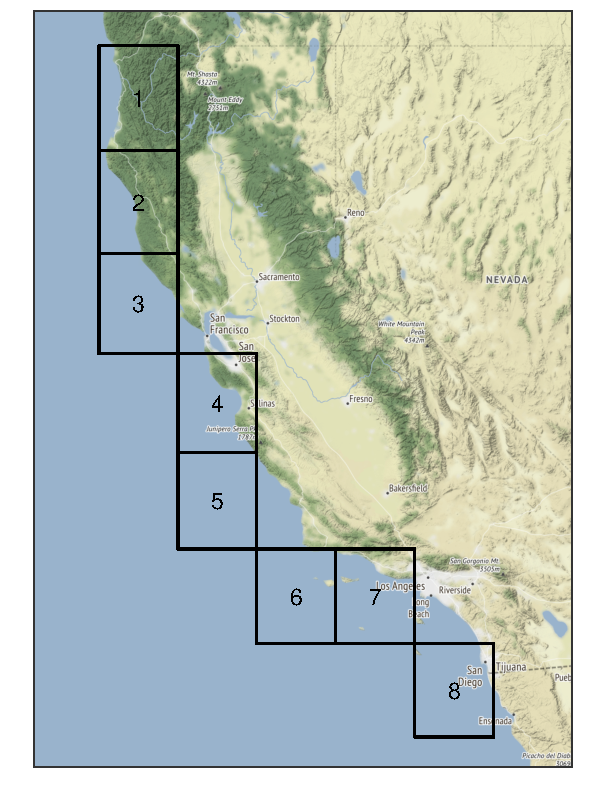
\includegraphics[width=0.99\linewidth]{./images/erai_grid}
    \end{minipage}%
    \begin{minipage}{0.25\textwidth}
    \centering
    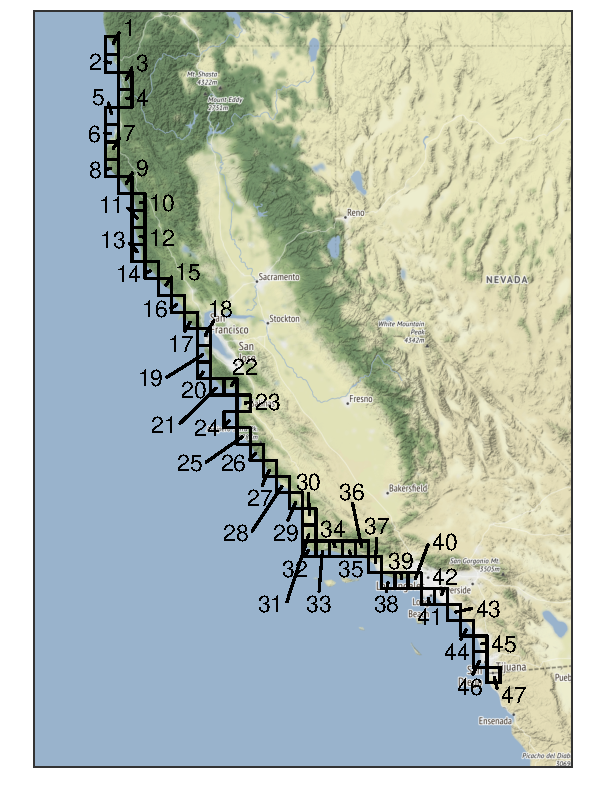
\includegraphics[width=0.99\linewidth]{./images/era5_grid}
    \end{minipage}
    \caption{Grid cell locations for ERA-Interim (left) and ERA5 (right).\label{fig:gridlocs}}
\end{figure}

Our data correspond to daily average values for the IVT magnitude
    along the coast of California.  The ERA-Interim data used covers the time period 
    1979 through 2014 (37 years) omitting leap days, and eight grid cells that 
    correspond to the coast of California.  The ERA5 data cover the time period 
    1979 through 2019 (42 years) with the same restriction, and  47 grid cells for 
    the coast of California.  This gives us the opportunity to illustrate the 
    performance of our method in multivariate settings of very different dimensions. 
    Figure~\ref{fig:gridlocs} provides a visual representation of the area these grid 
    cells cover.

\begin{algorithm}[htb]
    \caption{Data preprocessing to isolate and transform data exhibiting extreme behavior.  $r_i$
    represents the radial component, and $\bm{v}_i$ the angular component.  The declustering 
    portion is relevant for data correlated in time.\label{algo:processing}}
    \begin{algorithmic}
        \For{$\ell = 1,\ldots,d$}
            \State Set $b_{t,\ell} = \hat{F}_{\ell}^{-1}\left(1 - \frac{1}{t}\right)$.
            \State With $\bm{ x}_{\ell} > b_{t,\ell}$, fit $a_{\ell}$, $\xi_{\ell}$ via MLE according to generalized Pareto likelihood.
        \EndFor
        \For{$i = 1,\ldots,n$}
            \State Define $z_{i,\ell} = \left(1 + \xi_{\ell}\frac{x_{i,\ell} - b_{t,\ell}}{a_{\ell}}\right)_{+}^{1/\xi_{\ell}}$; $\;\;\;$ then $r_i = \pnorm{\bm{ z}_i}{\infty}$, $\;\;\bm{ v}_i = \frac{\bm{ z}_i}{\pnorm{\bm{ z}_i}{\infty}}$
        \EndFor
        \State Subset $\bm{ r},\bm{ v}$ such that $r_i \geq 1$
        \If{declustering}
            \For{$i = 1,\ldots,n$}
                \State If $r_i \geq 1$ and $r_{i-1} \geq 1$, drop the lesser (and associated $v_i$) from data set.
            \EndFor
        \EndIf
    \end{algorithmic}
\end{algorithm}


\begin{figure}[ht]%{l}{0.45\textwidth}
    \centering
    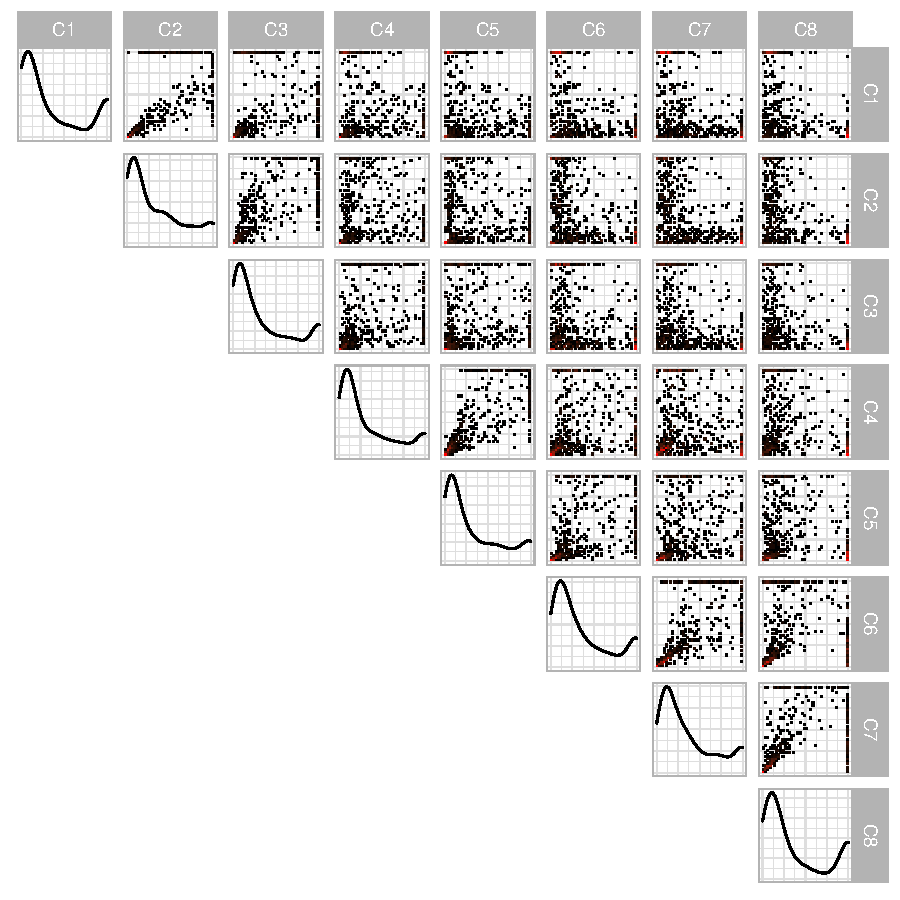
\includegraphics[width=.7\linewidth]{./images/data_transformed}
    \caption{Pairwise plots from ERA-Interim data after transformation and projection to ${\mathbb S}_{\infty}^{7}$.  Down the diagonal are marginal kernel densities, with two-dimensional histograms on the off-diagonal.  In those plots, red indicates a higher density.  All data is between 0 and 1.\label{fig:erai_data}}
\end{figure}

Fitting our models to the IVT data requires some pre-processing. First, we subset the data to the rainy
  season, which in California runs roughly from November to March.  Following the approach described 
  in Section \ref{sec:methodology} we estimate the shape and scale parameters of a univariate GP, in each
  dimension, using maximum likelihood. We set the threshold in each dimensions $\ell$ as  
  $b_{t,\ell} = \hat{F}_{\ell}^{-1}(1 - t^{-1})$, where $\hat{F}$ is the empirical CDF and $t=20$, 
  that corresponds to the $95$ percentile. We then use the transformation in Equation~\eqref{eqn:standardization} 
  to standardize the observations.  Dividing each standardized observation
  by its $\mathcal{L}_{\infty}$ norm, we obtain a projection onto $\mathcal{S}_{\infty}^{d-1}$. As 
  the data correspond to a daily time series, the observations are temporally correlated.  For each
  group of consecutive standardized vectors $z_i$ such  that  $\inorm{z_i} > 1$, we retain only the
  vector with the largest $\mathcal{L}_{\infty}$ norm.  The complete procedure is outlined in
  Algorithm~\ref{algo:processing}.  
  
After subsetting the ERA-Interim data to the rainy season we 
  have $5587$ observations. After the processing and declustering described in
  Algorithm~\ref{algo:processing}, this number reduces to $511$ observations. A pairwise plot 
  of the transformed data after processing and declustering is presented in 
  Figure~\ref{fig:erai_data}.  From this, we note that the marginal densities display strong
  similarities, with a large spike near 0 and a small spike near 1. A value of 1 in a particular 
  axis indicates that the standardized threshold exceedance was largest in that dimension.  
  The off-diagonal plots correspond to pairwise density plots.  We observe that some site pairs, such 
  as $(1,2)$, $(7,8)$, and especially $(4,5)$ have the bulk of their data concentrated in a 
  small arc along the $45^{\circ}$, while other site combinations such as $(3,6)$, $(2,7)$, or
  $(1,8)$ the data is split, favoring one side or the other of the $45^{\circ}$ line. For the 
  ERA5 data, after subsetting we have $6342$ observations, which reduces to $532$ observations 
  after processing and declustering. We fit the PG-G, PRG-G, PG-LN, and PRG-LN models to 
  both datasets.

% \begin{table}[htb]
%   \centering
%   \caption{Energy score criterion from fitted models against the IVT data. 
%     Lower is better.\label{tab:dev}}
%   
\begin{tabular}{cccccc}
\toprule
Source & pairwise_betas & sdpppg & sdpppgln & sdppprg & sdppprgln\\
\midrule
ERA-Interim & 0.8620 & 0.8003 & 0.7986 & 0.7966 & 0.7970\\
ERA5 & 2.0311 & 1.6404 & 1.5576 & 1.4349 & 1.5051\\
\bottomrule
\end{tabular}
% \end{table}

% \begin{table}[htb]
%   \centering
%   \caption{Time to sample (in minutes) 50,000 iterations for various models\label{tab:sampletime}}
%   \setlength\templen{\tabcolsep}
\setlength\tabcolsep{3.5pt}
\begin{tabular}{c|ccccc}
\toprule
Source & \begin{tabular}{@{}c@{}}Pairwise \\ Betas\end{tabular} & PG-G & PG-LN & PRG-G & PRG-LN\\
\midrule
ERA-Interim & $1.5$ & $16.3$ & $66.5$ & $14.8$ & $52.9$\\
ERA5 & $53.1$ & $19.4$ & $153.4$ & $24.6$ & $121.4$\\
\bottomrule
\end{tabular}
\setlength\tabcolsep{\templen}
% EOF
% \end{table}

\begin{table}[t]
    \centering
    \caption{Model fit assessment and computation time on ERA-Interim and ERA5 data.}
    \begin{subtable}{0.7\textwidth}
    \centering
    
\begin{tabular}{cccccc}
\toprule
Source & pairwise_betas & sdpppg & sdpppgln & sdppprg & sdppprgln\\
\midrule
ERA-Interim & 0.8620 & 0.8003 & 0.7986 & 0.7966 & 0.7970\\
ERA5 & 2.0311 & 1.6404 & 1.5576 & 1.4349 & 1.5051\\
\bottomrule
\end{tabular}
    \caption{Energy score criterion from fitted models against the IVT data. Lower is better.\label{tab:dev}}
    \end{subtable}
    \\
    \bigskip
    \begin{subtable}{0.7\textwidth}
    \centering
    \setlength\templen{\tabcolsep}
\setlength\tabcolsep{3.5pt}
\begin{tabular}{c|ccccc}
\toprule
Source & \begin{tabular}{@{}c@{}}Pairwise \\ Betas\end{tabular} & PG-G & PG-LN & PRG-G & PRG-LN\\
\midrule
ERA-Interim & $1.5$ & $16.3$ & $66.5$ & $14.8$ & $52.9$\\
ERA5 & $53.1$ & $19.4$ & $153.4$ & $24.6$ & $121.4$\\
\bottomrule
\end{tabular}
\setlength\tabcolsep{\templen}
% EOF
    \caption{Time to sample (in minutes) 50,000 iterations for various models\label{tab:sampletime}}
    \end{subtable}%
\end{table}



Table~\ref{tab:dev} shows the values of the estimated energy 
    scores for the different models considered. We observe that, contrary to the results in the
    simulation study in Figure~\ref{fig:simpples}, the preferred model is the projected restricted 
    gamma models, though for the lower-dimensional ERA-Interim data, all models perform comparably.
    Table~\ref{tab:sampletime} shows the computing times needed to fit the different models to the
    two datasets.  We see the effect of dimensionality on the various models; for gamma centered
    models it grows linearly; for the log-normal centered model, it will grow superlinearly as matrix
    inversion becomes the most costly operation.  For \verb|BMAmevt|, its parameter space grows
    combinatorically with the number of dimensions, and thus so does computational complexity and
    sampling time.
    % \bruno{Insert here the table that you sent me in the email and comment the results.}

\begin{figure}[b]
    \centering
    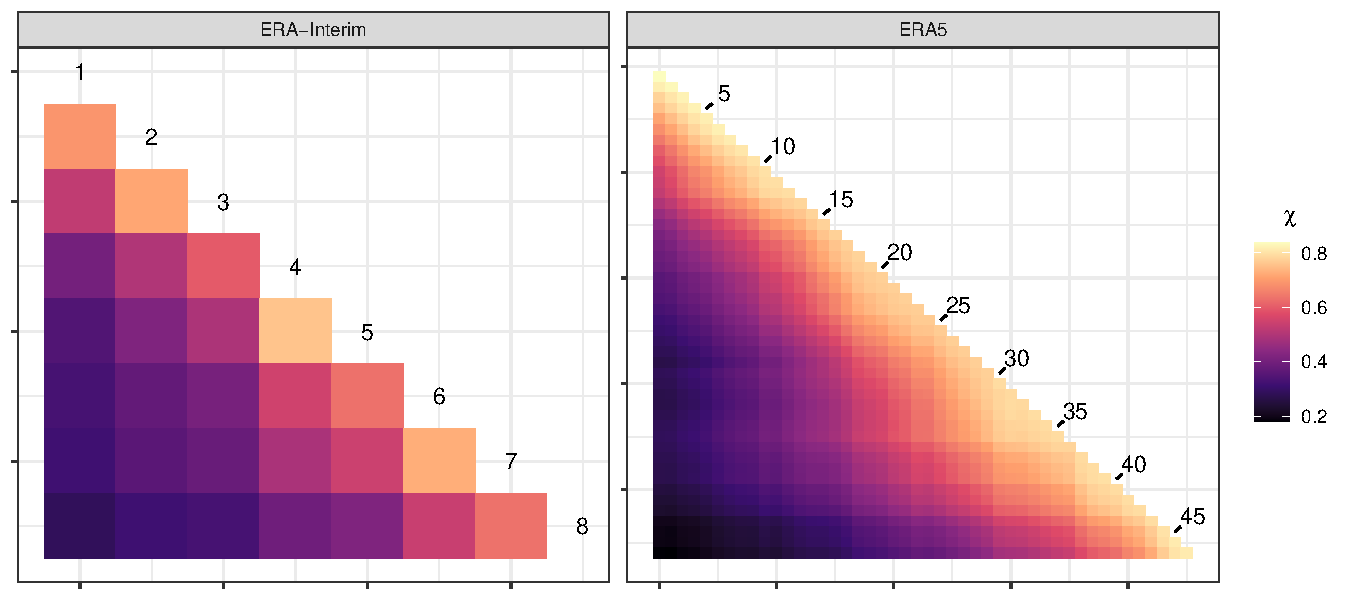
\includegraphics[width=0.9\textwidth]{./images/chi_ij_c}
    \caption{Pairwise extremal dependence coefficients for IVT data using the PRG-G model.\label{fig:chi_ij}}
\end{figure}

We consider an exploration of the pairwise extremal dependence using Monte Carlo estimates of the 
  coefficients in  Equation~\eqref{eqn:chi_ij}. For this we use samples obtained from the PRG-G model.
  Figure~\ref{fig:chi_ij} provides a graphical analysis of the results. 
  The coefficients achieve values between $0.286$ and $0.759$ for the ERA-Interim data and 
  between $0.181$ and $0.840$ for the ERA5 data.  The greater range in dependence scores observed 
  with the ERA5 data versus ERA-Interim speaks to the greater granularity of the ERA5 data,
  indicating that distance between locations is a strong contributor to the strength of the 
  pairwise asymptotic dependence. The highest coefficients are $0.759$ for 
  locations 4 and 5 in the ERA-Interim data and
  $0.840$ for locations 1 and 2 in the ERA5 data.  Clearly, pairwise asymptotic
  dependence coefficients tell a limited story, as a particular dependence may include
  more than two locations.   We can, however, glean some information from the patterns that
  emerge in two dimensions.  For the ERA-Interim data, we observe a possible cluster 
  between cells 5-8, indicating a strong dependence among these cells.  Analogously, for
  the ERA5 data, we observe three possible groups of locations.

\begin{figure}[t]
    \centering
    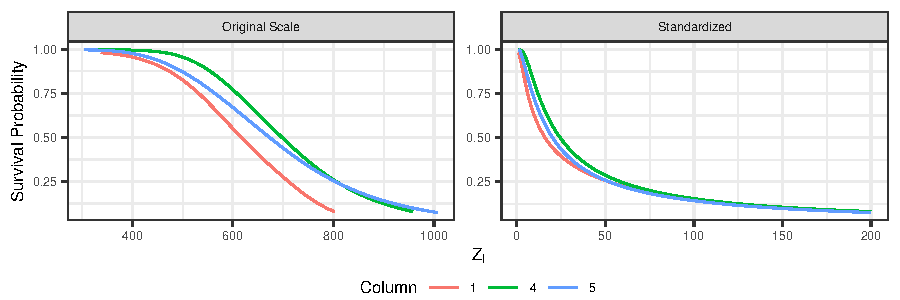
\includegraphics[width=\linewidth]{./images/condsurv_1d}
    \caption{Conditional survival curves for selected locations, using ERA-Interim, and PRG-G model,  conditioning on all other dimensions at greater than 90th percentile (fitted)\label{fig:condsurv1d}. The left panel uses original units. Right panel uses standardized units.}
\end{figure}

\begin{figure}[t]
    \centering
    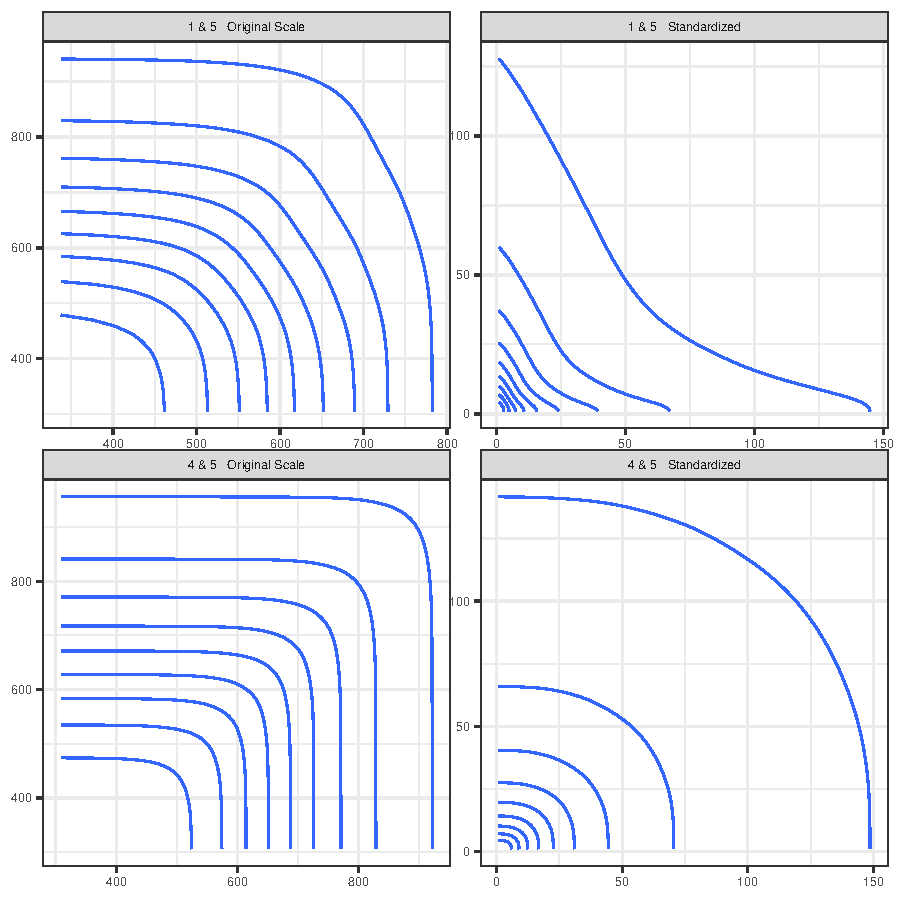
\includegraphics[height=4in, width=4in]{./images/condsurv_2d}
    \caption{Pairwise conditional survival curves for selected locations, using 
        ERA-Interim, and PRG-G model, conditioning on all other dimensions at greater 
        than 90th percentile (fitted).\label{fig:condsurv2d}}
\end{figure}

Figure~\ref{fig:condsurv1d} shows, for the ERA-Interim data under the PRG-G model,  
    the conditional survival curve defined in Equation~\eqref{eqn:condsurv}, for one dimension, 
    conditioned on all other dimensions being greater than their (fitted) $90$th percentile. 
    Figure~\ref{fig:condsurv2d} presents the bi-variate conditional survival function,
    conditioning on all other dimensions.  These results illustrate quantitatively how 
    extremal dependence affects the shape of the conditional survival curves.  The two 
    top panels represent the joint survival function 
    between grid locations 4 and 5, which are shown in Figure~\ref{fig:chi_ij} to exhibit 
    strong  extremal dependence.  We observe that the joint survival surface 
    is strongly convex.  The bottom panels represent the joint survival surface between 
    grid locations 1 and 5, which exhibited low extremal dependence.  In this case the 
    shape of the contours tend to be concave, quite different from the shapes observed 
    in the top panels.

Using our proposed scoring criteria, we explored the effect of the choice of $p$ on the 
    final results. Using the simulated data, generated from a mixture of projected Gammas, 
    we were unable to observe sizeable differences in the scores for $p$ ranging between 
    1 and 15.   However, for the IVT data, we observed a drop in the energy score associated 
    with higher $p$, with diminishing effect as $p$ increased.  We observed no significant 
    differences in the performance of the model that uses $p=10$, which corresponds to the 
    analysis presented, relative to the one that uses $p=15$.
% EOF
